\documentclass{ieeeaccess}
\usepackage{cite,amsmath,amssymb,amsfonts,graphicx,booktabs,array,url,bm}
\usepackage{needspace}
\def\BibTeX{{\rm B\kern-.05em{\sc i\kern-.025em b}\kern-.08em T\kern-.1667em\lower.7ex\hbox{E}\kern-.125emX}}
\begin{document}
\vol{XX}\year{XXXX}
\history{}
\doi{}
\title{Protocol-Constrained Residual Adaptation for Rigid-Body Inference: A Bounded Evaluation of Frozen Visual Features}
\author{\uppercase{Hyojin Park}\authorrefmark{1}, \uppercase{Nam-Hyun Yoo}\authorrefmark{2}, and \uppercase{Jinhong Yang}\authorrefmark{3}}
\address[1]{Gyeongnam Intelligence Innovation Center (GIIC), Kyungnam University, 7, Gyeongnamdaehak-ro, Masanhappo-gu, Changwon 51767, Republic of Korea}
\address[2]{Computer Engineering, Kyungnam University, Changwon 51767, Republic of Korea}
\address[3]{Department of Medical Information Technology, Inje University, Gimhae 50834, Republic of Korea}
\tfootnote{}
\markboth{Park \headeretal: Protocol-Constrained Residual Adaptation}{Park \headeretal: Protocol-Constrained Residual Adaptation}
\corresp{Corresponding author: Jinhong Yang (e-mail: jinhong@inje.ac.kr).}
\begin{abstract}
Inferring rigid-body properties from short videos requires separating motion-supported information from learned corrections. We study a protocol-constrained residual adapter anchored to a fixed robust numerical estimate. A numerical ridge update is followed by a smaller visual residual from a frozen vision encoder and observation decoder. Corrections are bounded in anchor-standard-deviation units and restricted to permitted physical coordinates. On new synthetic geometry families, the complete adapter reduces analytic new-action error by 29.95\% relative to the one-step-weight Huber anchor. A post hoc comparison with iteratively converged Huber fitting retains a 24.11\% reduction. Most improvement comes from numerical adaptation in sliding protocols. The additional visual increment is 1.07\%, with a two-sided 95\% interval that includes zero; cross-fitted residual targets retain its direction. Development-selected channel controls attribute the measured signal primarily to decoder position corrections, without isolating a benefit of language pretraining. A controlled engine-rollout proxy preserves the improvement and closely tracks the analytic metric. Task-specific fitting on a public pushing dataset also retains improvement when both object and surface friction conditions are held out, within the same object and scene assets. Proper scores improve, while empirical coverage remains conservative. These findings support numerical-first residual correction and a bounded, task-dependent contribution from the tested visual view. They do not establish calibrated posterior guarantees or real-world property transfer.
\end{abstract}
\begin{keywords}
physical parameter estimation, residual learning, rigid-body dynamics, robust estimation, uncertainty evaluation, frozen visual features.
\end{keywords}
\titlepgskip=-15pt
\maketitle

\section{Introduction}\label{sec:introduction}
\PARstart{S}{hort} videos can support several explanations of the same motion. Mass, friction, restitution, initial conditions, image tracking errors, and camera geometry interact in an inverse problem. Predicting a plausible property from appearance is therefore different from identifying a property that explains an observed intervention. This distinction matters when an inferred state is used to predict a subsequent action.

Physical prediction and hybrid estimation have been studied through controlled video benchmarks and structured model corrections \cite{bear2021physion,tung2023physionpp,yin2021aphynity,revach2022kalmannet}. Recent quantitative benchmarks extend this agenda to numerical properties \cite{puyin2026quantiphy,zhan2026idpp}. The unresolved question addressed here is narrower: after a strong numerical path has consumed a short motion observation, does a compact frozen visual feature view provide additional predictive information?

We use a fixed robust anchor, a numerical residual head, and a bounded visual residual head. The visual features are produced by the frozen vision component of Qwen3-VL-2B-Instruct and a previously trained observation decoder that is frozen for the reported residual experiments \cite{bai2025qwen3vl}. The method does not generate a language description or update the foundation-model weights. A protocol mask limits which transformed physical coordinates may change. One bounce convention disables the complete correction. A positive-semidefinite covariance increment accompanies the accepted mean displacement; it is an uncertainty heuristic whose quality must be measured.

The contribution is a concrete residual-estimation design and its controlled evaluation. The design assigns most adaptation to numerical inputs, restricts the visual update in protocol-permitted coordinates, and retains an explicit numerical-only comparator. The evaluation separates three questions: whether the complete adapter improves fixed robust estimators on a new-geometry parameter-to-trajectory benchmark; whether the selected visual view adds information after matched numerical adaptation; and how the resulting approximate distributions behave under proper scores and empirical coverage. The paper does not propose a new ridge solver, a general identifiability theorem, or a new foundation model.

The main error reduction is 29.95\% against the one-step-weight Huber anchor and 24.11\% against a post hoc iteratively converged Huber fit, whereas the original visual increment is 1.07\%. A separate public simulator dataset yields a 4.27\% visual-plus-gate increment after task-specific readout fitting. These percentages describe different estimands and cannot be combined into a single transfer effect. The public experiment failed its original 10\% development threshold, and the real-video diagnostic did not establish transfer. We retain both boundaries while evaluating the positive method results.

The four deliverables of this study are:
\begin{itemize}
\item A numerical-first residual allocation with protocol masks, anchor-scale clipping, and accepted-update covariance inflation.
\item A matched numerical comparator that separates the selected visual increment from the complete-model gain.
\item A new-geometry evaluation under locally specified effect-size, directional, and protection-cell rules.
\item An inspectable evidence package that includes unsuccessful development criteria, transfer boundaries, and reproducible post hoc component analyses.
\end{itemize}

\section{Related Work}\label{sec:related}
\subsection{Quantitative Evidence and Identifiability}
Physion and Physion++ evaluate physical prediction, including cases in which latent object properties affect the outcome \cite{bear2021physion,tung2023physionpp}. Differentiable physical reasoning has also combined video, language, and a physics model \cite{li2021dvr}. QuantiPhy evaluates numerical physical quantities, while the dynamic-property study of Zhan \emph{et al.} compares classical visual evidence, video-model readouts, and multimodal prompting \cite{puyin2026quantiphy,zhan2026idpp}. These tasks motivate evaluating additional visual information against a strong motion estimator.

Recent preprints examine the difference between supplied evidence and learned priors: Ill-Posed by Design probes evidence use, and EquiSD uses scale equivariance to train metric grounding \cite{meivar2026illposed,tan2026equisd}. Our coordinate mask is a restricted protocol rule. It does not solve general monocular identifiability or establish that all masked coordinates coincide with a measured Jacobian null space.

\subsection{VLM-Assisted Physical Inference}
NeRF2Physics connects language-embedded spatial features to physical properties, while PhysX-Anything generates simulation-ready assets from images \cite{zhai2024nerf2physics,cao2026physxanything}. These appearance-oriented settings differ from predicting the consequence of a short dynamic intervention.

Phys2Real fuses VLM physical priors with online interaction estimates and evaluates real manipulation \cite{wang2026phys2real}. RigPI combines VLM initialization and search-space constraints with force--torque and motion measurements in differentiable simulation \cite{he2026rigpi}. $\Delta$ynamics uses a structured language representation for video-based rigid-body dynamics \cite{kao2026dynamics}. Table~\ref{tab:related} identifies methodological distinctions; it is not a performance ranking across incompatible tasks. The recent Code as Worlds preprint further explores executable representations \cite{wang2026codeworlds}. Our contribution concerns the limited residual role assigned to a particular frozen feature view after numerical adaptation.

\begin{table*}[t]
\caption{Position Relative to Closely Related Methods; Different Sensing and Tasks Preclude a Direct Accuracy Ranking}
\label{tab:related}\centering\small
\begin{tabular}{p{.12\textwidth}p{.24\textwidth}p{.27\textwidth}p{.27\textwidth}}
\toprule Method & Information and representation & Role of physical computation & Evaluation boundary \\ \midrule
Phys2Real \cite{wang2026phys2real} & Visual physical priors and robot interaction estimates & Online adaptation with uncertainty-aware fusion & Real manipulation; different sensing and policy objective \\
RigPI \cite{he2026rigpi} & VLM semantic initialization, force--torque, and motion & Differentiable parameter refinement in a constrained search space & Real parameter-identification tasks; cited as a 2026 preprint \\
$\Delta$ynamics \cite{kao2026dynamics} & Video and structured textual dynamics representation & Structured dynamics inference & Video-based rigid-body prediction; no matched experiment here \\
This work & Eight frames, known setup inputs, numerical features, frozen observation-decoder features & Fixed robust anchor and bounded residual heads; no added solver loop & Synthetic analytic actions and an offline public displacement task; real transfer unresolved \\
\bottomrule\end{tabular}
\end{table*}

\subsection{Residual Estimation and Frozen Features}
APHYNITY separates a physical model from a learned correction, and KalmanNet combines structured estimation with neural components \cite{yin2021aphynity,revach2022kalmannet}. Residual learning and hybrid estimation are thus established ideas. Huber weighting and ridge regression supply the robust and regularized components used here \cite{huber1964robust,hoerl1970ridge}; Theseus illustrates a broader differentiable-optimization approach \cite{pineda2022theseus}.

BLIP-2 demonstrates lightweight adaptation of frozen components \cite{li2023blip2}. V-JEPA 2 and V-JEPA 2.1 provide motion-oriented representations \cite{assran2025vjepa2,murlabadia2026vjepa21}. An additional V-JEPA 2 control uses the same eight observations, numerical anchor, and residual-stage dimension and rules. Its upstream supervision and spatial processing differ from the Qwen-derived decoder view. It is therefore a frozen-representation comparison, not a fully matched intervention on language pretraining or semantic physical knowledge.

\subsection{Selective Use and Uncertainty}
Answer-Level Trust Selection studies selective use of quantitative physical answers \cite{yu2026ats}. Our public gate instead scales a vector correction. Neither an average gate value nor lower mean error proves calibrated confidence. Negative log-likelihood (NLL) and the continuous ranked probability score (CRPS) evaluate predictive distributions jointly with coverage and width \cite{gneiting2007proper}. Formal conformal guarantees require a compatible procedure and assumptions \cite{angelopoulos2023conformal}; the development-residual quantile used here is reported as empirical, without such a guarantee. The August--September 2026 papers above are explicitly treated as recent preprints, not settled evidence of superiority.

\section{Problem and Evaluation Definition}\label{sec:problem}
\begin{table}[htbp]\centering\small
\caption{Terminology Used in This Study}\label{tab:terms}
\begin{tabular}{p{.28\columnwidth}p{.62\columnwidth}}\toprule
Term & Operational meaning\\\midrule
Protocol & Specified motion/contact regime and permitted coordinates.\\
Convention & Assumed bounce setup information; slides are shared.\\
Complete model & Numerical and visual residuals, including fixed fallback.\\
Numerical view & Motion, setup, prior and initialization features.\\
Analytic action error & Parameter-to-trajectory projection under fixed new inputs.\\
Protection cell & A convention/protocol point-error harm check.\\
\bottomrule\end{tabular}
\end{table}

The main physical state is
\begin{equation}
\bm\theta=[\log(m/\mathrm{kg}),\log\mu,\operatorname{logit}e]^\top,
\end{equation}
where $m$, $\mu$, and $e$ denote mass, dynamic friction, and restitution. An observation model has the form $\bm o=h_p(\bm\theta;\bm u,\bm\eta)+\bm\epsilon$, with known protocol inputs $\bm u$ and nuisance variables $\bm\eta$. For ideal horizontal sliding during a fixed contact regime, $a=F/m-\mu g$ explains why distinct known forces can separate mass and friction, whereas unforced deceleration alone does not identify mass. This idealized argument motivates the coordinate permissions in Table~\ref{tab:protocol}; it is not a conditioning guarantee for noisy image data.

\begin{table}[t]\caption{Main Protocol Permissions and Assumptions}\label{tab:protocol}\centering\small\setlength{\tabcolsep}{3pt}
\begin{tabular}{>{\raggedright\arraybackslash}p{.23\columnwidth}>{\raggedright\arraybackslash}p{.32\columnwidth}>{\raggedright\arraybackslash}p{.34\columnwidth}}
\toprule Protocol & Known inputs and nuisance & Permitted correction \\ \midrule
Multiple-force slide & Two force values and switch time; initial position/velocity nuisance & $\log m,\log\mu$ \\
Unforced slide & Zero applied force; initial position/velocity nuisance & $\log\mu$ \\
General bounce & Gravity 9.81 m/s$^2$; initial height, velocity, floor nuisance & $\operatorname{logit}e$ permitted by protocol, but final residual disabled \\
Setup bounce & Known release height 0.65 m and zero initial velocity; free common offset & $\operatorname{logit}e$ \\
\bottomrule\end{tabular}\end{table}

The two conventions differ in their treatment of bounce setup information. Generalized translation permits initial height, velocity, and floor nuisance variables with fixed gravity. Setup translation uses the known release height and zero initial velocity and profiles a common vertical offset. Slide inference is shared. Averaging both conventions is a specified benchmark aggregation, not two independent experimental replications. Camera geometry, motion noise, force, and prior inputs belong to this controlled setup; arbitrary RGB-only deployment is not evaluated.

Protocol permission and final fallback are distinct operations: the bounce protocol permits a restitution coordinate, whereas the generalized-bounce branch subsequently suppresses its entire learned correction. A supplementary audit summarizes the saved initialization Jacobians after nuisance projection; it does not equate protocol permissions with the null space of an unrestricted model.

The main action metric uses an independent NumPy implementation of canonical analytic trajectories, not a new PyBullet or PhysX rollout. Estimated and true properties generate trajectories under the same new action, at eight times from 0.125 to 1.0 s. Multiple-force sliding uses forces $(0.45,1.1)$ N with a 0.35 s switch and initial velocity 0.25 m/s; unforced sliding starts at 1.0 m/s; bounce starts at 0.85 m. Mean absolute position error is averaged within each family/protocol, then equally across three protocols, two conventions, and 72 families. The images come from synthetic geometry scenes; analytic action utility must be distinguished from engine-rollout accuracy.

The synthetic observation renderer uses PyBullet~\cite{coumans2022pybullet}. The public task predicts a planar displacement vector using an offline onset-aligned video selection. It is a different output from the transformed-property distribution. Its target, timestamp audit, and information-access limitations are defined in Section~\ref{sec:protocol}.

\Needspace{6\baselineskip}
\section{Method}\label{sec:method}
\subsection{Fixed Robust Anchor and Feature Construction}
A fixed Huber-weighted numerical fit produces mean $\bm a_{ir}$ and covariance $\bm C_{ir}$ for episode $i$ and convention $r$. Standardized innovations from an initial unit-weight update determine $w_t=\min(1,1.345/|\nu_t|)$. Observation standard deviations are replaced by $\sigma_t/\sqrt{w_t}$ before the nonlinear fit. These weights are computed once, rather than repeatedly recomputed as a converged Huber M-estimator. The Cauchy control uses $w_t=[1+(\nu_t/2.385)^2]^{-1}$. The underlying solver retains the specified priors, nuisance handling, and fixed dispersion scale. The covariance is a local curvature approximation; contact/start-selection uncertainty is not integrated out. Detailed code locations are supplied in the supplement.

The numerical view $\bm x_i^N\in\mathbb R^{192}$ flattens 24 channels at eight frames: active-axis position, relative position, finite-difference velocity and velocity difference, log observation noise, time, time increment, time from force switch, switch indicator, two forces, switch time, three active-coordinate flags, three prior means, three log prior scales, and three normalized linearization coordinates. It excludes the selected Qwen-derived residual channels, but includes known setup and prior information. It is not an uncontrolled image-only baseline.

All compared primary paths share a frozen appearance prior. A first-image Qwen forward pass with a fixed appearance-description prompt supplies a final-token representation to a learned linear mean/scale head. Thus ``numerical only'' denotes the residual head's feature restriction, not an absence of VLM computation throughout the pipeline. The overall gain measures residual adaptation conditional on this common prior; the visual increment isolates the additional eight-frame feature view. The prior stage uses the language-model representation, while the additional visual residual path does not generate text. The supplement distinguishes these upstream stages and their training scope.

The visual path uses the last pre-merge states of the Qwen vision encoder: a $32\times32$ grid with 1,024 features per frame. Frames are processed separately at a $512^2$ pixel budget with BF16 vision computation. A previously trained, frozen observation decoder fuses those states with RGB, tracking, an initial bounding box, and temporal transport. Its attention-weighted 32-channel states, captured before the static/dynamic position heads, supply eight pooled vectors. No text prompt or language-decoder state is used in this extraction. The 48-dimensional residual view concatenates their temporal mean with eight dynamic and eight static position corrections normalized by tracking noise. Thus the features are VLM-derived observation-decoder features, rather than 32 directly selected language-model channels.

\subsection{Sequential Residual Training and Inference}
Let $\bm s_{ir}=\sqrt{\operatorname{diag}(\bm C_{ir})}$. Separate ridge heads are fitted for each protocol and convention, using only that protocol's active output coordinates. For a training feature matrix $\bm X$, each channel is centered and divided by its training standard deviation, floored at $10^{-6}$. Let $\tilde{\bm X}$ denote the standardized matrix and $\bar{\bm y}$ the training target mean. Each head solves
\begin{equation}
\bm W_\lambda=\arg\min_{\bm W}\left\{\|\tilde{\bm X}\bm W-(\bm Y-\bm 1\bar{\bm y}^{\top})\|_F^2+\lambda\|\bm W\|_F^2\right\}.
\label{eq:ridge}
\end{equation}
Its prediction is $f(\bm x)=\bm W_\lambda^\top\tilde{\bm x}+\bar{\bm y}$; the intercept is unpenalized. The loss is a sum, not a sample-averaged loss, which fixes the meaning of the reported penalties. Numerical targets are $(\bm\theta_i-\bm a_{ir})\oslash\bm s_{ir}$, where $\oslash$ denotes elementwise division. The numerical prediction is clipped before forming the visual target:
\begin{align}
\bm z^N_{irp}&=\operatorname{clip}(f^N_{rp}(\bm x_i^N),-2,2),\\
\bm z^V_{irp}&=\operatorname{clip}(f^V_{rp}(\bm x_i^V),-1,1).
\end{align}
Ridge penalties are 1 and 10, respectively. If $\bm a^N_{ir}=\bm a_{ir}+\bm s_{ir}\odot(\bm M_{ip}\bm z^N_{irp})$, the visual training target is $(\bm\theta_i-\bm a^N_{ir})\oslash\bm s_{ir}$ on the active coordinates. Thus the visual target uses the numerical head's \emph{in-sample training prediction}. Feature normalization, target centering, and both fits use the outer training families only. The complete pair is evaluated on the outer held-out family fold. Cross-fitted numerical training targets would define a different estimator and are not used here.

With diagonal protocol mask $\bm M_{ip}$, the mean update is
\begin{equation}
\hat{\bm\theta}_{ir}=\bm a_{ir}+\bm s_{ir}\odot\left[\bm M_{ip}(\bm z^N_{irp}+0.25\bm z^V_{irp})\right].\label{eq:update}
\end{equation}
For generalized bounce, development observations of harmful learned correction motivated setting the full correction to zero; this fallback was fixed before confirmation. Removing the visual term elsewhere retains the numerical correction; it does not return the original anchor. Sequential refers to target construction: both fitted heads can be evaluated from their feature views at inference.

The stored weights and intercepts number $2(2+1+1)[(192+1)+(48+1)]=1,936$. Of these, 242 belong to generalized-bounce heads whose outputs are discarded, leaving 1,694 potentially active coefficients across the other branches. These counts exclude the foundation model, previously trained observation decoder, normalization statistics, and the public extension. They describe residual-stage capacity. On 100 batch-one episodes, median residual-head time is 0.342 ms, whereas the sum of measured inference components is 362.5 ms on an RTX 5080; the supplement specifies the staged timing scope. A development sensitivity sweep retains the original shrinkage 0.25 without confirmation-set reselection. Collapsing repeated setup channels to an 87-dimensional numerical view is reported separately as a post hoc variant.

\subsection{Approximate Uncertainty}
For the accepted correction $\bm d=\hat{\bm\theta}-\bm a$,
\begin{equation}
\hat{\bm\Sigma}=\bm C+\operatorname{diag}[(0.1\bm d)^2].\label{eq:cov}
\end{equation}
The addition is positive semidefinite. It depends on the complete accepted correction magnitude, not an independently estimated disagreement probability. The clipping bounds imply $|d_j|\leq2.25s_j$, so $\hat\Sigma_{jj}\leq1.050625C_{jj}$ and the marginal standard deviation increases by less than 2.5\%. This is a coordinatewise bound, not a guarantee on all correlated ellipsoid axes or on coverage.

NLL and marginal Gaussian CRPS are computed in transformed-property space on the protocol's active principal covariance submatrix. A joint region contains the target when its squared Mahalanobis distance is below the 90th percentile of a chi-square distribution with the active dimension. Scores and joint-axis diameters use family/protocol macro aggregation. These quantities evaluate parameter uncertainty. With the complete mean fixed, inflation changes NLL by only $-0.0135$ nats per active dimension; CRPS is lowest without inflation, and point error is unchanged.

\begin{figure*}[t]\centering
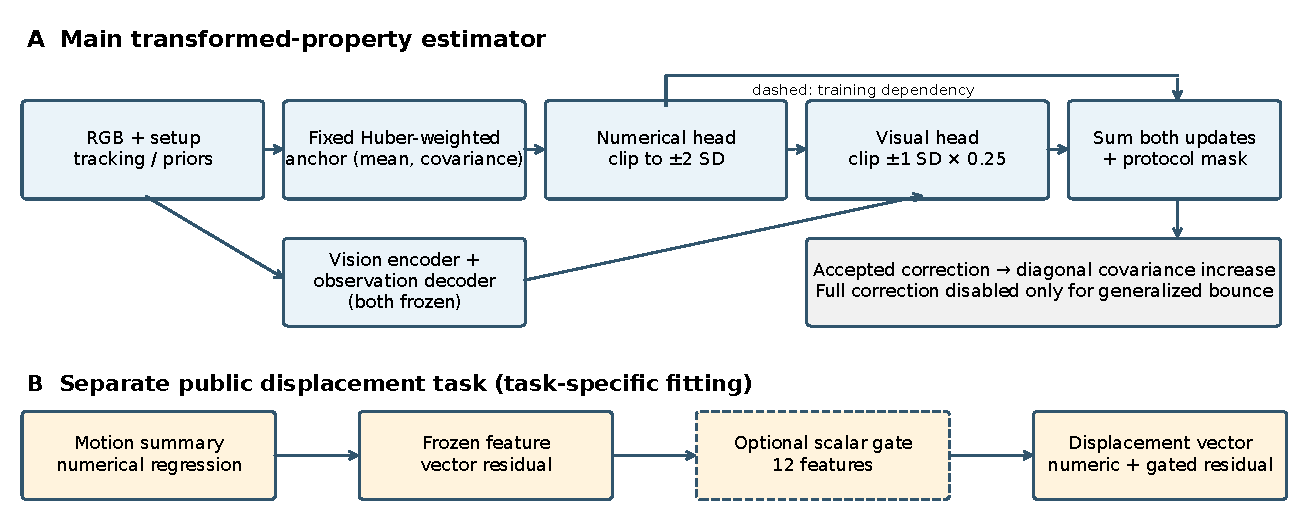
\includegraphics[width=\textwidth]{figures/fig1_architecture.pdf}
\caption{Main residual estimator and separate public-task extension. All primary paths share the first-image learned prior supplied to the fixed anchor. Training dependencies are distinguished from prediction outputs. Disabling only visual correction retains numerical adaptation; complete anchor fallback applies to generalized bounce. The public displacement head has neither the main property mask nor its covariance-inflation rule.}\label{fig:architecture}
\end{figure*}

\subsection{Public Displacement Head and Gate}
The public extension predicts a two-dimensional displacement in meters, rather than a physical-property distribution. It fits a ridge-regularized numerical regression with iterative Huber-style residual weighting on an 11-dimensional motion summary, followed by a 144-dimensional visual temporal-feature regression on its in-sample residuals. The selected numerical, visual, and gate penalties are 10, 1,000, and 0.1, respectively. Numerical weighting is recomputed for at most 50 iterations; this differs from the main anchor's fixed innovation weights. Visual corrections are norm-clipped to the development target-norm standard deviation, 0.067724 m for the final fit. A scalar quality gate produces
\begin{equation}
\hat{\bm y}_i=\hat{\bm y}_i^N+g_i\Delta\hat{\bm y}_i^V,\qquad 0\leq g_i\leq1.\label{eq:gate}
\end{equation}
Its 12 inputs summarize tracking/decoder disagreement, temporal feature variation, object-size stability, prediction and correction magnitudes, and their alignment. Four-fold cross-fitting inside each of five outer folds generates component predictions used to train an optimal-scalar target:
\begin{equation}
g_i^*=\operatorname{clip}\!\left(\frac{(\bm y_i-\hat{\bm y}_i^N)^\top\Delta\hat{\bm y}_i^V}{\max(\|\Delta\hat{\bm y}_i^V\|^2,10^{-12})},0,1\right).
\end{equation}
The target minimizes squared vector error along a fixed correction; model selection uses mean Euclidean displacement error, denoted vector mean absolute error (MAE). For episode errors $e_i=\|\hat{\bm y}_i-\bm y_i\|_2$, the reported MAE is $n^{-1}\sum_i e_i$ and root mean squared error (RMSE) is $\sqrt{n^{-1}\sum_i e_i^2}$. Neither is the componentwise mean absolute error. Five gate penalties are compared using the outer predictions. Because component choices and gate penalties were selected using the same development cohort, this is cross-fitting of gate targets, not a fully nested unbiased estimate of all model selection.

The selected out-of-fold radial errors supply the 90\% radius, using rank $\lceil(53+1)0.9\rceil=49$. The same 53 episodes participate in fitting, selection, and residual calibration. The procedure is neither independent split conformal nor an implemented CV+/jackknife+ construction. We therefore report an empirical development-calibrated radial region. The final models and radius are fixed before public confirmation scoring. A valid future split-conformal design would require a calibration partition excluded from fitting and selection. A 20-episode calibration sample would have rank resolution $1/21$ and 90\% rank 19; small size makes estimation coarse but does not itself invalidate split conformal. We do not repartition the already evaluated cohort to claim new independent calibration.

\section{Experimental Protocol}\label{sec:protocol}
\subsection{Development and New-Geometry Confirmation}
The residual candidate was selected using 132 development geometry families and six-fold family cross-fitting. Its development action-error reduction was 31.61\% against the strongest fixed robust estimator; the visual increment was 1.44\%.\footnote{The development cohort includes the 720 episodes used to train the upstream observation decoder. These six folds isolate residual fitting only and are not equivalent to the new-geometry confirmation.} The local plan required at least 10\% complete-model improvement, positive paired visual direction, proper-score guards, joint 90\% coverage within an author-defined 85--98\% range, and bounded width and protocol harm. Candidate configuration and checkpoint were locally locked before generation of the new confirmation cohort. Hashes establish content identity; they are not public preregistration or independent proof of chronology.

The new cohort contains 72 geometry families, 1,080 episodes, and 8,640 frames. All episodes are scored. Stored records report prediction sealing before target opening and no subsequent fitting or exclusions. We replay the saved statistical inputs here; we do not claim a new end-to-end training run or independent reconstruction of every access event.

Controls are unit, Huber, and Cauchy weighting, a frozen legacy observation adapter, an RGB temporal control, and the matched numerical residual. The latter removes the visual head while retaining the anchor, numerical head, protocol mask, and accepted-update covariance rule. Family losses are resampled in 20,000 paired draws. In each draw, the robust reference is the minimum sampled mean among the three fixed robust methods. The primary rule combines a point improvement of at least 10\% with a negative one-sided 95\% upper bound; it does not establish a population improvement lower bound of 10\%. Six cell guards use the better cell error of the globally strongest robust method and the legacy adapter, with both 10\% relative and 0.10 mm absolute harm limits. These are engineering protection criteria, not six simultaneous confidence guarantees.

\subsection{Offline Public Dataset Task}
PhysProbe Push was obtained at the pinned dataset commit identified in the supplement, associated with Isaac Sim 4.5 and Isaac Lab 2.2.1 \cite{mittal2025isaaclab,physprobe2026dataset}. A fixed episode selection excluded feasibility episodes 0--9 and assigned 64 candidate episodes to development and 128 to confirmation. An RGB eligibility procedure retained 53 and 123. The split is by episode; shared physical-parameter, object, or environment groups have not been established as independent across these roles.

The saved video headers and parquet timestamps agree on 50 fps for all 176 retained episodes. Frame offsets are $[-21,-16,-11,-6,-1,4,9,14]$ around detected onset. The target is the planar position at onset+90 minus the position at onset. Thus the last observation is 0.28 s after onset, the target endpoint is 1.80 s after onset, and the remaining horizon is 1.52 s. This is displacement from onset, not displacement starting at the last observation. Source frames are resized to $280\times280$ for the decoder path.

The extraction program tracks the red component across the complete video before determining eligibility and onset. Failure on a later frame can exclude an episode. Although selected features use only eight frames and do not read simulator targets, cohort selection uses future video availability. We therefore describe an offline, onset-aligned, visibility-selected benchmark, not validated causal online forecasting. The timing audit does not eliminate selection bias or establish object-group independence.

The public development search produced a 3.90\% improvement and did not pass its original 10\% threshold. A narrower secondary directional hypothesis and an empirical coverage guard were recorded before the 123 confirmation trajectories were scored. We preserve that history and do not use 4.27\% to retroactively pass the development threshold. Episode-bootstrap intervals use 100,000 stored paired draws. Their interpretation assumes episode exchangeability and does not substitute for an unperformed physical-group analysis.

Reporting the failed development criterion makes the subsequent secondary direction interpretable and prevents retrospective threshold adjustment.

\begin{figure*}[t]\centering
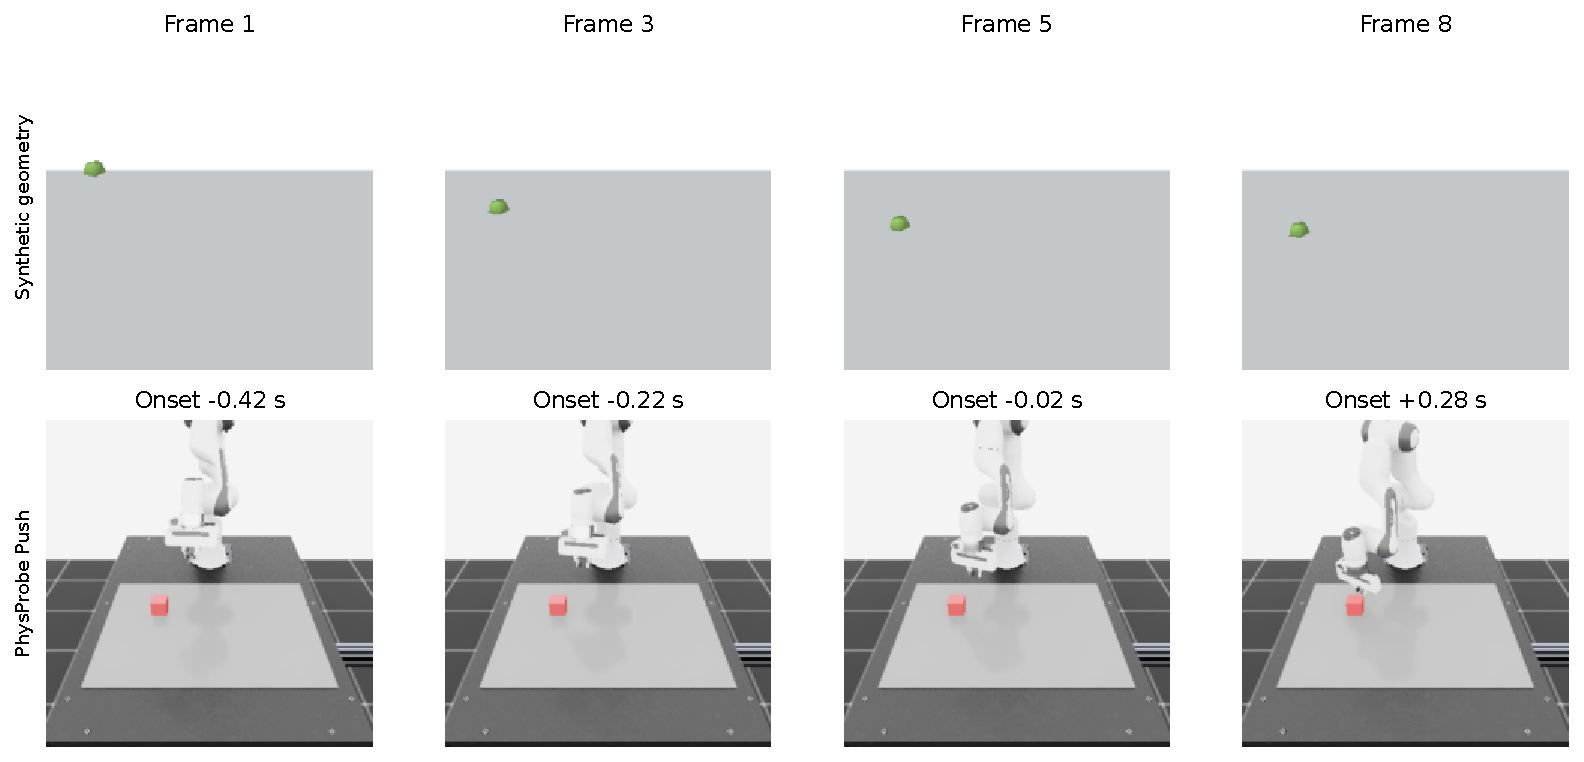
\includegraphics[width=\textwidth]{figures/fig4_observation_samples.pdf}
\caption{Representative inputs from the synthetic geometry and public pushing tasks. Four of eight selected frames are shown; synthetic insets enlarge the tracked object while retaining the complete scene. Public time labels are relative to detected onset at the verified 50 fps cadence; no metric scale is inferred from the image alone.}\label{fig:observations}
\end{figure*}

\section{Results}\label{sec:results}
\subsection{Complete Model and Visual Increment}
The complete adapter obtains 1.453 mm analytic action MAE, versus 2.074 mm for the strongest fixed robust point baseline (Table~\ref{tab:main}). The reduction computed from full-precision records is 29.95\%. The primary draw-wise-strongest comparison has a one-sided upper bound of $-0.459$ mm. These results satisfy the original main effect-size and directional rules.

An explicit replay finds that Huber has the lowest sampled robust mean in all 20,000 draws. This explains why the draw-wise-strongest and fixed-Huber intervals coincide for these saved samples; it is not an identity assumed by the comparison rule.

\begin{table}[t]\caption{New-Geometry Analytic Action Error (72 Families)}\label{tab:main}\centering
\begin{tabular}{lrr}\toprule Method & MAE (mm) & Relative to Huber\\\midrule
Unit weighting & 2.119 & $+2.16\%$\\
Huber weighting & 2.074 & reference\\
Cauchy weighting & 2.081 & $+0.34\%$\\
Legacy observation adapter & 2.151 & $+3.71\%$\\
RGB temporal control & 2.384 & $+14.95\%$\\
Numerical residual & 1.469 & $-29.19\%$\\
\textbf{Numerical + visual residual} & \textbf{1.453} & $\mathbf{-29.95\%}$\\\midrule
\multicolumn{3}{l}{\emph{Post hoc baselines; outside original rules}}\\
Iterated Huber & 1.915 & $-7.69\%$\\
Iterated Cauchy & 1.913 & $-7.76\%$\\
Profiled-dispersion MAP & 1.823 & $-12.11\%$\\
Direct ridge & 33.403 & $+1510.3\%$\\
Direct MLP (3-seed mean) & 26.489 & $+1177.0\%$\\\bottomrule
\end{tabular}\par\small Direct regressors predict transformed coordinates without an anchor update or output mask and do not supply a posterior.\end{table}

Numerical adaptation explains most of the gain. Adding the visual residual gives a further 1.07\%. Its one-sided 95\% upper bound is $-0.00219$ mm, while its two-sided interval is $[-0.03114,+0.00053]$ mm and includes zero. We report both, rather than describing an unqualified two-sided significant visual effect. This is an ablation of the selected combined feature view, not proof of semantic physical knowledge.

A descriptive family-level sensitivity analysis provides complementary information about effect concentration. The complete model improves on fixed Huber in 56 of 72 families; the visual increment improves on the numerical residual in 46 of 72. The median paired visual difference is $-0.01117$ mm. Leaving out any single family retains a negative visual mean difference, ranging from $-0.01995$ to $-0.01346$ mm. The exact two-sided sign test gives $p=0.02446$, while the mean-difference bootstrap interval includes zero. These test different hypotheses: directional frequency can be consistent even when a small mean effect is sensitive to asymmetric magnitudes. Both are reported; the post hoc sign test does not replace the primary mean analysis.

The six recorded rows contain three distinct, nontrivial protection comparisons: multiple-force sliding, unforced sliding, and setup bounce. Duplicate slide rows share inference, while generalized bounce is equal by construction at 0.515 mm. All three nontrivial checks pass. They share families and are not statistically independent replications.

\begin{figure*}[t]\centering
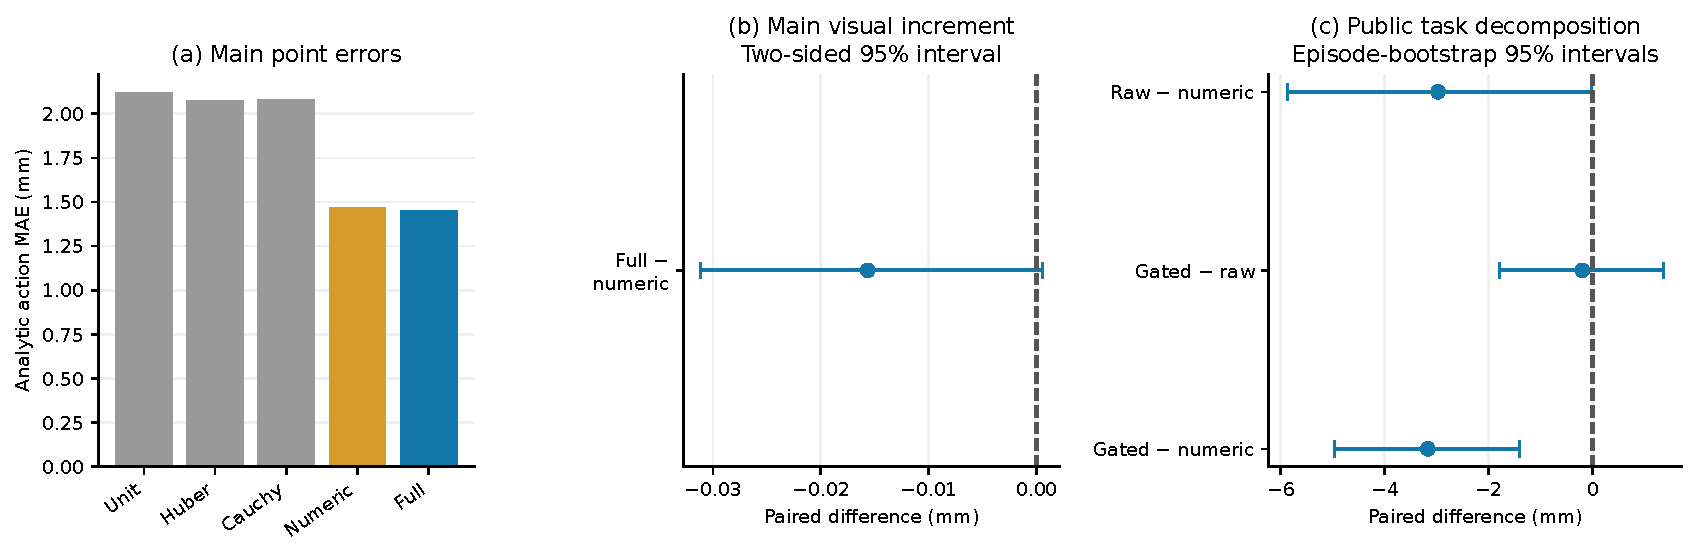
\includegraphics[width=\textwidth]{figures/fig2_main_results.pdf}
\caption{Point errors and paired effect intervals. The public contrasts separating raw residual and gate are post hoc diagnostics; the complete public contrast replays the original paired draws. Each axis labels its own range; the paired differences use substantially different scales. Negative paired differences favor the candidate.}\label{fig:results}
\end{figure*}


\paragraph{Baseline strength and allocation of gain}
All newly added comparisons are post hoc and outside the original analysis rules. The original model is evaluated unchanged. Iterated Huber and Cauchy fits update residual-based weights until convergence, preserving the original physical prior and nuisance bounds; a concentrated Gaussian likelihood additionally profiles dispersion. Their errors are 1.915, 1.913, and 1.823 mm, respectively. Full-minus-iterated-Huber error is $-0.4617$ mm with an unadjusted paired 95\% interval of $[-0.6634,-0.2698]$ mm, retaining 24.11\% improvement. The corresponding profiled-MAP reduction is 20.30\%. These nonlinear fits are local solutions, not global-optimum guarantees. The supplement reports iteration counts, nonconverged cases, and all paired intervals. Direct ridge and a small direct MLP selected on development families have substantially larger point errors in this implementation.
\begin{table}[htbp]\centering\small
\caption{Protocol Breakdown in Millimeters; Iterated Huber Is Post Hoc}\label{tab:breakdown}
\begin{tabular}{lrrrr}\toprule
Protocol & Fixed H. & Iterated H. & Numeric & Full\\\midrule
Multiple forces & 3.633 & 3.068 & 3.020 & 2.990\\
Unforced slide & 2.156 & 2.087 & 0.978 & 0.960\\
General bounce & 0.515 & 0.834 & 0.515 & 0.515\\
Setup bounce & 0.352 & 0.345 & 0.301 & 0.304\\
\bottomrule\end{tabular}
\end{table}

Against the original cell-specific best-of-robust/legacy reference, sliding contributes 99.9\% of the macro error reduction; unforced sliding, whose only corrected coordinate is $\log\mu$, contributes 61.8\%. That reference differs from the single Huber row in Table~\ref{tab:main}. The six-cell mean and coordinate-specific errors are reproduced in the supplement. The concentration in sliding is compatible with correction of systematic anchor error; the present design does not fully separate this mechanism from acquisition of additional information.

\paragraph{Target construction and channel attribution}
Five inner family folds generate out-of-fold numerical predictions for visual training targets, with penalties, clipping, and shrinkage unchanged. The post hoc cross-fitted variant yields 1.45162 mm on the previously evaluated families: a 1.17\% visual increment with paired interval $[-0.03446,+0.00095]$ mm. Direction is retained, but the interval again includes zero. No confirmation outcomes select this variant.
\begin{table}[htbp]\centering\small
\caption{Post Hoc Channel Controls with Development-Selected Penalties}\label{tab:channels}
\begin{tabular}{lrrr}\toprule
View & Penalty & Develop. & Evaluated\\\midrule
Combined & 10 & 1.3522 & 1.4531\\
Pooled states & 1 & 1.3671 & 1.4675\\
Position shifts & 1 & 1.3512 & 1.4511\\
\bottomrule\end{tabular}
\end{table}

Each channel view uses the same development search over penalties $\{1,10,100\}$. Pooled states alone yield 1.46746 mm, close to the 1.46877 mm numerical comparator. Position shifts yield 1.45112 mm; their post hoc difference from numerical prediction is $-0.01765$ mm with unadjusted interval $[-0.03101,-0.00512]$ mm. The combined view retains penalty 10 and the original result. This evidence is compatible with tracking-related decoder information and does not isolate a language-pretraining contribution. The groups share the same upstream trained decoder.

Disabling generalized-bounce fallback worsens the full-model error by $0.04165$ mm, with paired interval $[0.03078,0.05253]$ mm. Thus this learned correction is harmful in the tested branch; fallback is a measured limitation of the adapter rather than a universal safety guarantee.

\paragraph{Engine-rollout proxy}
A post hoc PyBullet proxy applies the same new actions to estimated and true properties of a nonrotating sphere. Huber, numerical, and full errors are 2.236, 1.620, and 1.606 mm. The full reduction relative to Huber is 28.19\%; family-level Spearman correlations with the analytic metric range from 0.961 to 0.986. This supports agreement of rankings under the controlled contact proxy, while the primary metric remains a parameter-to-trajectory projection. It does not validate rollouts of the original geometry assets or real manipulation.

\subsection{Proper Scores and Conservative Coverage}
Table~\ref{tab:uncertainty} reports the active transformed-property scores. The full mean-and-covariance estimate improves NLL and CRPS over the robust baseline. Its joint 90\% coverage is 97.36\%, exceeding nominal coverage by 7.36 percentage points. This is consistent with covariance that is too broad relative to the corrected errors. Passing the 85--98\% engineering guard is distinct from matching nominal coverage. The mean joint-axis width ratio is 1.002 relative to Huber. Since the mean and covariance change together, these results do not isolate a causal benefit of the inflation rule.

\begin{table}[t]\caption{Transformed-Property Distribution Evaluation}\label{tab:uncertainty}\centering
\begin{tabular}{lrrr}\toprule Method & NLL/dim. & CRPS & 90\% coverage\\\midrule
Huber & $-2.372$ & 0.01755 & 0.9343\\
Numerical residual & $-2.542$ & 0.01314 & 0.9736\\
Numerical + visual & $-2.546$ & 0.01311 & 0.9736\\\bottomrule
\end{tabular}\end{table}



\subsection{Public Displacement and Gate Decomposition}
The public numerical predictor obtains 74.182 mm vector MAE. The raw visual residual yields 71.210 mm, and gating yields 71.015 mm (Table~\ref{tab:public}). The complete visual-plus-gate increment is 4.27\%, with paired difference $-3.167$ mm and episode-bootstrap 95\% interval $[-4.957,-1.400]$ mm. This supports the recorded secondary direction within the selected offline cohort, subject to the episode-exchangeability limitation.

\begin{table}[t]\caption{Public Displacement Error in Millimeters (123 Held-Out Episodes)}\label{tab:public}\centering
\begin{tabular}{lrrr}\toprule Method & MAE & Median & RMSE\\\midrule
Constant prior & 132.132 & 117.007 & 145.861\\
Numerical & 74.182 & 63.054 & 89.584\\
Raw visual residual & 71.210 & 61.252 & 84.631\\
Gated visual residual & 71.015 & 58.338 & 85.006\\\bottomrule
\end{tabular}\end{table}

Mean target displacement is 193.869 mm (median 215.989 mm). Numerical, raw, and gated normalized MAEs are 0.383, 0.367, and 0.366; their vector $R^2$ values are 0.621, 0.662, and 0.659. The development-mean constant prior has $R^2=-0.0044$, providing a scale sanity check.

The gate alone changes MAE by $-0.195$ mm (0.274\%), with post hoc 95\% interval $[-1.785,+1.360]$ mm. Its RMSE increases from 84.631 to 85.006 mm. The gate is therefore an optional quality weighting in these results, not an established source of significant improvement. The raw-visual-versus-numerical interval is $[-5.872,-0.025]$ mm; this additional decomposition is also post hoc and unadjusted for multiple comparisons.

The gate-only change improves 52 episodes, worsens 64, and leaves seven unchanged. Its leave-one-episode-out mean difference ranges from $-0.507$ to $+0.074$ mm, so even its mean direction is sensitive to an individual episode. By contrast, the complete gated-versus-numerical mean remains negative in every such deletion. These are descriptive post hoc diagnostics; the originally selected gated model is retained without confirmation-set reselection.

Empirical radial 90\% coverage is 96.75\% for the gated model and 95.93\% for numerical prediction. Isotropic Gaussian NLL changes from $-2.612$ to $-2.691$; the isotropic scale is derived from the fixed radial radius. The mean gate of 0.545 describes correction amplitude, not confidence calibration. External readouts were fitted on PhysProbe development targets, so this is task-specific adaptation to another simulator dataset rather than zero-shot transfer of a physical-property posterior.

\subsection{Real-Video Boundary}
A public real-friction diagnostic uses 33 videos from 11 object--surface families in a pre-existing test partition \cite{zhan2026idpp}. This diagnostic defines a boundary on transfer claims rather than evidence of practical deployment. The short-window feature score exhibits an inverse family association: Spearman $-0.70$, with the recorded family-bootstrap interval $[-0.972,-0.108]$. This is a directional failure of that score, not merely an absent positive result. A source audit finds a feature-unit mismatch: synthetic position shifts are noise-normalized, whereas the real diagnostic uses axis-projected pixel shifts. Its output is a residual score, not an inferred friction coefficient, and the appearance prior is not used. Pooled-only correlation is 0.027 and position-only correlation is $-0.455$. These observations identify a domain/measurement mismatch, but do not isolate a causal explanation of failure. A separately developed, 152-frame kinematic bridge produces Spearman $0.355$, Pearson $0.682$, and macro pair accuracy 0.693 across five object/camera comparison groups (21 pairs). Its permutation $p=0.1423$ does not establish transfer. A scalar kinematic proxy reaches Spearman $0.427$, exceeding the bridge's rank correlation. The bridge changes both information and observation duration; it cannot rescue a claim of direct frozen-feature transfer.

\subsection{Additional Material-Disjoint Public Evaluation}\label{sec:group}
A metadata audit identifies 16 object-friction pairs and 16 surface-friction pairs in PhysProbe Push. The original eligible development and evaluation sets share 15 object-material and all 16 surface-material conditions. Thus the original episode split is not material-disjoint. All episodes use the same red cube; friction conditions are metadata scalars without corresponding material-identifying appearance cues in this setup. The result tests generalization of motion summaries across friction conditions, not recognition of material from appearance or transfer to distinct object/scene assets.

We fixed a follow-up protocol before reading new videos or displacement targets. It excludes all 202 previously selected or feasibility episodes and assigns eight object materials and eight surface materials to evaluation. Training uses the complementary materials on both axes; mixed assignments are omitted. The unchanged visibility procedure retains 285 training and 329 evaluation episodes from 320 and 348 candidates. The evaluation spans 63 of 64 possible held-out material pairs. No object- or surface-friction pair is shared between fitting and evaluation, and no complete video hash is shared. The original architecture and penalties are retained, with newly fitted coefficients. Internal gate targets also exclude both materials of each held-out pair. Evaluation trajectories are downloaded only after predictions are sealed.

Equal weighting of the 63 material-pair mean errors yields 63.419 mm for numerical prediction and 60.641 mm for the gated residual, a 4.38\% reduction (Table~\ref{tab:group}). The paired difference is $-2.778$ mm, with a two-way material-bootstrap 95\% interval of $[-6.044,-0.116]$ mm. Marginal differences favor the candidate in seven of eight object-material groups and five of eight surface-material groups. These outcomes satisfy the locally fixed directional and group-consistency rule. The interval's upper endpoint is close to zero, and eight groups per axis limit precision. This validates the fitted readout under held-out friction conditions within the same cube/scene setting. Architecture selection previously used episodes from this material bank; the study does not establish historically untouched material discovery, new object-asset transfer, or a causal online evaluation. The original 3.90\% development failure and 4.27\% episode-split result remain separate records.

\begin{table}[t]\caption{New-Episode Evaluation with Both Material Axes Held Out (329 Episodes)}\label{tab:group}\centering
\begin{tabular}{lrr}\toprule Method & Material-pair MAE & Episode MAE\\\midrule
Numerical & 63.419 & 65.091\\
Raw visual residual & 61.943 & 64.642\\
Gated visual residual & 60.641 & 62.753\\\bottomrule
\end{tabular}
\par\small Both columns are in millimeters. Material-pair MAE is the primary metric and weights observed material combinations equally. Episode MAE is descriptive. Episode-normalized errors are 0.342, 0.340, and 0.330; vector $R^2$ values are 0.634, 0.649, and 0.657. Mean target displacement is 190.281 mm.
\end{table}

\subsection{Post Hoc Component and Covariance Analyses}\label{sec:component}
The supplement provides the complete cached-feature ablations, covariance sweep, and additional development sensitivity results. Original models remain fixed. In particular, the 87-dimensional numerical-view variant removes repeated setup channels and selects its penalty on development families; its descriptive evaluated error is 1.42632 mm. This sensitivity shows that feature duplication changes effective regularization, without retroactively replacing the primary configuration.

The additional frozen V-JEPA 2 control yields 1.470615 mm on the previously evaluated cohort, versus 1.468770 mm for numerical-only and 1.453122 mm for the original full model. The V-JEPA-minus-full paired interval is $[-0.00118,+0.03560]$ mm. Thus the full model has a lower point error, but this post hoc comparison does not establish a two-sided superiority claim. Training-fold-only PCA supplies 48 video features; no additional frames, target-dependent projection, or model reselection is used. The supplement reports development scores and distinct upstream processing costs. Development comparisons are structurally unmatched because only the Qwen observation decoder was trained on part of that cohort; the evaluated cohort also cannot isolate pretraining without matched upstream supervision.

\section*{Data and Code Availability}
Verification materials are provided in release v0.3.0 of \url{https://github.com/Jinhong-Yang/physics-residual-verification}. The Overleaf project includes source, figure data, selected observations and predictions, residual checkpoints, and executable calculation/refitting tools. New post hoc baseline, cross-fitting, channel, shrinkage, direct-regression, engine, scale, and diagnostic results are supplied with their plans and numerical inputs. The RGB companion reproduces eight complete inference paths, including the shared appearance prior, after separately obtaining hash-checked foundation weights. Recorded latency summaries can be replayed; fresh hardware measurement additionally needs the measurement source's original 100-episode RGB inputs and upstream environment. Full upstream training is not reproduced. The public dataset is available at the pinned repository in \cite{physprobe2026dataset}.

\section{Discussion}\label{sec:discussion}
The strongest supported contribution is protocol-constrained numerical residual correction. Its improvement persists against iteratively converged local robust estimators, but is smaller than the fixed-anchor headline. Channel controls localize the smaller visual signal primarily to position corrections. Table~\ref{tab:scope} collects the main inferential boundaries.
\begin{table*}[htbp]\centering\small
\caption{Evidence Established and Limits of the Present Design}\label{tab:scope}
\begin{tabular}{p{.45\textwidth}p{.45\textwidth}}\toprule
Supported within the tested setting & Not established\\\midrule
Sliding residual adaptation improves fixed and iterated anchors. & Separation of anchor bias correction from additional information.\\
Cross-fitted visual targets retain a small mean improvement. & A two-sided full-view effect or a language-pretraining benefit.\\
Refitting generalizes across both friction-condition axes. & Transfer to unseen object or scene assets.\\
Proper scores improve with broad empirical regions. & Nominally calibrated posterior coverage.\\
The tested real-video score fails directionally. & A causal explanation or general impossibility of real transfer.\\
\bottomrule\end{tabular}
\end{table*}

Generalized bounce illustrates the boundary of learned correction. Across development folds, predicted-versus-true standardized residual correlations range from $-0.202$ to 0.231, compared with 0.429--0.658 for setup bounce. On evaluated episodes, correlations are 0.186 and 0.502; generalized-bounce target standard deviation is 2.264 versus 0.571. Anchor-scale medians are similar (0.00752 versus 0.00710), so large median covariance inflation alone does not explain failure. The wider residual-target dispersion and weaker predictability are consistent with the greater nuisance freedom; this observational diagnosis does not isolate its causal effect. Visual clipping activates on 6.39\% of generalized-bounce predictions and none of the setup-bounce predictions.

The adapter is small, but its complete computation is not characterized by coefficient count. Measured median component totals are 362.5 ms with the additional visual path and 129.1 ms for the shared-prior/RGB-anchor path; these are sums across staged, model-resident runs rather than contiguous cold-start latency. First-image prior computation and the additional vision encoder dominate the budget, while the residual heads require 0.342 ms. Removing all VLM computation would also remove the common prior and would define a different baseline.

The positive datasets are synthetic. The friction holdout retains the original material-bank architecture-selection history and shared cube/scene assets. The analytic metric and controlled engine proxy do not test the original geometry assets in an independent downstream manipulation task. Unmatched upstream supervision, independent calibration, complete upstream training reproduction, and the real-video feature-unit mismatch remain substantive limits. No model or hyperparameter is reselected on the previously evaluated cohorts.

\section{Conclusion}\label{sec:conclusion}
Protocol-constrained residual adaptation reduces trajectory-projection error primarily through numerical correction of sliding estimates; improvement remains against iterated robust fitting. The tested visual view retains a small directional increment under cross-fitted targets, with position-correction channels accounting for most of its measured signal. Learned correction is harmful in generalized bounce and requires the fixed fallback. Neither language-pretraining benefit, nominal posterior calibration, nor successful real-video property transfer is established. The next evaluation should equalize upstream supervision across encoders and reserve an independent calibration split. Object/scene-asset holdouts should test the reach of the material-condition result. Prospective causal video selection and consistent physical feature units are needed before interpreting real-world deployment.

\section*{Acknowledgment}
This work was supported by the Institute of Information \& Communications Technology Planning \& Evaluation (IITP) -- Innovative Human Resource Development for Local Intellectualization program grant funded by the Korea government (MSIT) (IITP-2026-RS-2024-00436773).

OpenAI Codex (GPT-6) was used in literature discovery, verification-code development, and \LaTeX{} editing. Human authors are responsible for the scientific content and reference verification. Tool information: \url{https://openai.com/codex/}.

\bibliographystyle{IEEEtran}\bibliography{references}
\par\noindent\begin{minipage}{\columnwidth}\begin{IEEEbiography}[{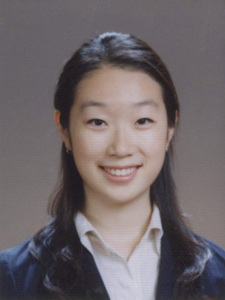
\includegraphics[width=1in,height=1.25in,clip,keepaspectratio]{authors/Hyojin-Park.png}}]{Hyojin Park}
received the Ph.D. degree in information and communications engineering from the Korea Advanced Institute of Science and Technology (KAIST), South Korea, in August 2024. Since 2025, she has been a Researcher with the Gyeongnam Intelligence Innovation Center (GIIC) at Kyungnam University. In 2020, she founded TOVDATA Inc., a privacy management technology company, where she also conducted related research. Her current research interests include Physical AI and Physics-Informed Neural Networks (PINNs). ORCID: \url{https://orcid.org/0009-0002-2387-8994}.
\end{IEEEbiography}\end{minipage}\par
\par\noindent\begin{minipage}{\columnwidth}\begin{IEEEbiography}[{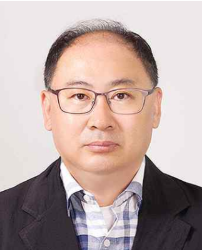
\includegraphics[width=1in,height=1.25in,clip,keepaspectratio]{authors/namhyun-yoo.png}}]{Nam-Hyun Yoo}
was a Postdoctoral Researcher with the AI SuperLab, Department of Computer Engineering, University of Oklahoma, USA, from September 2008 to February 2010. Since March 2013, he has been an Associate Professor with the Department of Computer Engineering, College of Engineering, Kyungnam University, South Korea. He has also served as an Expert Member of ISO TC184/SC 5 (Industrial Automation Systems Integration) since April 2022 and as the Director of the Gyeongnam Intelligence Innovation Project Group since July 2024. His research interests include manufacturing intelligence, Physical AI, and Embodied AI.
\end{IEEEbiography}\end{minipage}\par
\par\noindent\begin{minipage}{\columnwidth}\begin{IEEEbiography}[{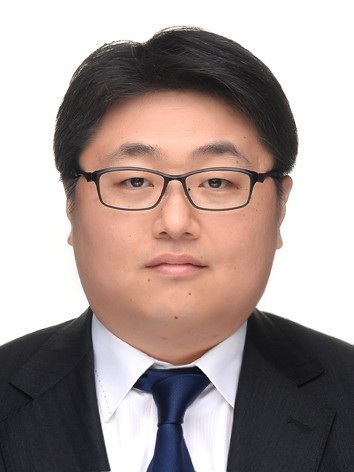
\includegraphics[width=1in,height=1.25in,clip,keepaspectratio]{authors/jinhong-yang.png}}]{Jinhong Yang}
received the Ph.D. degree in Information and Communication Engineering from KAIST. He was the Chief Technology Officer (CTO) with HECAS Inc. In March 2018 he joined Inje University, South Korea, as an Associate Professor. His research interests include vision-language models (VLMs), physics-informed neural networks, and AI agents. ORCID: \url{https://orcid.org/0000-0002-7756-0263}.
\end{IEEEbiography}\end{minipage}\par
\EOD
\end{document}
